\documentclass[a4paper,12pt]{article}

\usepackage{float}

\usepackage[normalem]{ulem}
\useunder{\uline}{\ul}{}

\usepackage[utf8]{inputenc}
\usepackage[dvips]{graphicx}
%\usepackage{a4wide}
\usepackage{epsfig}
\usepackage{fancybox}
\usepackage{verbatim}
\usepackage{array}
\usepackage{latexsym}
\usepackage{alltt}
\usepackage{amssymb}
\usepackage{amsmath,amsthm}
\usepackage{bm}
\usepackage{wasysym}

%\usepackage{fullpage}
%\usepackage{hyperref}
\usepackage{listings}
\usepackage{color}
\usepackage{algorithm}
\usepackage{algpseudocode}
\usepackage[hmargin=2cm,vmargin=3.0cm]{geometry}
%\topmargin=0cm
%\topmargin=-1.8cm
%\addtolength{\textheight}{6.5cm}
%\addtolength{\textwidth}{2.0cm}
%\setlength{\leftmargin}{-3cm}
%\setlength{\oddsidemargin}{0.0cm}
%\setlength{\evensidemargin}{0.0cm}

%misc libraries goes here
\usepackage{tikz}
\usepackage{tikz-qtree}
\usetikzlibrary{automata,positioning}

\usepackage{multicol}
\usepackage{enumitem}

\usepackage[most]{tcolorbox}

\usepackage[colorlinks=true,urlcolor=black,linkcolor=black]{hyperref}


\lstdefinestyle{customtex}{
    %backgroundcolor=\color{lbcolor},
    tabsize=2,
    language=TeX,
    numbers=none,
    basicstyle=\footnotesize\ttfamily,
    numberstyle=\footnotesize,
    aboveskip={0.0\baselineskip},
    belowskip={0.0\baselineskip},
    %
    columns=flexible,
    keepspaces=true,
    fontadjust=true,
    upquote=true,
    %
    breaklines=true,
    prebreak=\raisebox{0ex}[0ex][0ex]{\ensuremath{\hookleftarrow}},
    frame=single,
    showtabs=false,
    showspaces=false,
    showstringspaces=false,
    %
    %identifierstyle=\color[rgb]{0,0.2,0.8},
    identifierstyle=\color[rgb]{0,0,0.5},
    %identifierstyle=\color[rgb]{0.133,0.545,0.133},
    %keywordstyle=\color[rgb]{0.8,0,0},
    %keywordstyle=\color[rgb]{0.133,0.545,0.133},
    keywordstyle=\color[rgb]{0,0,0.5},
    %commentstyle=\color[rgb]{0.133,0.545,0.133},
    commentstyle=\color[rgb]{0.545,0.545,0.545},
    %stringstyle=\color[rgb]{0.827,0.627,0.133},
    stringstyle=\color[rgb]{0.133,0.545,0.133},
    %
    literate={â}{{\^{a}}}1 {Â}{{\^{A}}}1 {ç}{{\c{c}}}1 {Ç}{{\c{C}}}1 {ğ}{{\u{g}}}1 {Ğ}{{\u{G}}}1 {ı}{{\i}}1 {İ}{{\.{I}}}1   {ö}{{\"o}}1 {Ö}{{\"O}}1 {ş}{{\c{s}}}1 {Ş}{{\c{S}}}1 {ü}{{\"u}}1 {Ü}{{\"U}}1 {~}{$\sim$}{1}
}

\lstdefinestyle{output}{
    %backgroundcolor=\color{lbcolor},
    tabsize=2,
    numbers=none,
    basicstyle=\footnotesize\ttfamily,
    numberstyle=\footnotesize,
    aboveskip={0.0\baselineskip},
    belowskip={0.0\baselineskip},
    %
    columns=flexible,
    keepspaces=true,
    fontadjust=true,
    upquote=true,
    %
    breaklines=true,
    prebreak=\raisebox{0ex}[0ex][0ex]{\ensuremath{\hookleftarrow}},
    frame=single,
    showtabs=false,
    showspaces=false,
    showstringspaces=false,
    %
    %identifierstyle=\color[rgb]{0.44,0.12,0.1},
    identifierstyle=\color[rgb]{0,0,0},
    keywordstyle=\color[rgb]{0,0,0},
    commentstyle=\color[rgb]{0,0,0},
    stringstyle=\color[rgb]{0,0,0},
    %
    literate={â}{{\^{a}}}1 {Â}{{\^{A}}}1 {ç}{{\c{c}}}1 {Ç}{{\c{C}}}1 {ğ}{{\u{g}}}1 {Ğ}{{\u{G}}}1 {ı}{{\i}}1 {İ}{{\.{I}}}1   {ö}{{\"o}}1 {Ö}{{\"O}}1 {ş}{{\c{s}}}1 {Ş}{{\c{S}}}1 {ü}{{\"u}}1 {Ü}{{\"U}}1
}

\lstset{style=customtex}


\tikzset{%
    terminal/.style={draw, rectangle,
    				 align=center, 
					 minimum height=1cm, 
					 minimum width=2cm,
					 fill=black!10,
					 anchor=mid},
    nonterminal/.style={draw, rectangle,
    					align=left,
					    minimum height=1cm, 
						minimum width=2cm, 
						anchor=mid},% and so on
}

%% Style for terminals
%\tikzstyle{terminal}=[draw, rectangle, 
%					  minimum height=1cm, 
%					  minimum width=2cm, 
%					  fill=black!20,
%					  anchor=south west]
%% Style for nonterminals
%\tikzstyle{nonterminal}=[draw, rectangle, 
%						 minimum height=1 cm, 
%						 minimum width=2 cm, 
%						 anchor=north east]


\newcommand{\HRule}{\rule{\linewidth}{1mm}}
\newcommand{\kutu}[2]{\framebox[#1mm]{\rule[-2mm]{0mm}{#2mm}}}
\newcommand{\gap}{ \\[1mm] }

\newcommand{\Q}{\raisebox{1.7pt}{$\scriptstyle\bigcirc$}}
\newcommand{\minus}{\scalebox{0.35}[1.0]{$-$}}

\setlength{\fboxsep}{10pt}

\tcbsetforeverylayer{enhanced jigsaw, breakable, arc=0mm, boxrule=1pt, boxsep=5pt, after=\vspace{1em}, colback=white, colframe=black}

\newcolumntype{P}[1]{>{\centering\arraybackslash}p{#1}}

\setlength\parindent{0pt}

%\renewcommand\arraystretch{1.2}

\newenvironment{Tab}[1]
  {\def\arraystretch{1}\tabular{#1}}
  {\endtabular}

%%%%%%%%%%%%%%%%%%%%%%%%%%%%%%%%%%%%%%%%%%%%%%%%%%%%%%%%%%%%%%%%%%%%%%%%%%%%%%%%%%%%%%

\title{Formal Languages and Abstract Machines \\ Take Home Exam 2}
\author{Ugur Duzel \\ 2171569} % write your name and id
\date{} % do not write any date

%%%%%%%%%%%%%%%%%%%%%%%%%%%%%%%%%%%%%%%%%%%%%%%%%%%%%%%%%%%%%%%%%%%%%%%%%%%%%%%%%%%%%%

\begin{document}
\HRule\\
Middle East Technical University \hfill Department of Computer Engineering
{\let\newpage\relax\maketitle}
\HRule\\
\vspace{1cm}

%%%%%%%%%%%%%%%%%%%%%%%%%%%%%%%%%%%%%%%%%%%%%%%%%%%%%%%%%%%%%%%%%%%%%%%%%%%%%%%%%%%%%%

% Write your answers below the section tags
\section{Context-Free Grammars \hfill \normalfont{(10 pts)}}

\paragraph{a)} Give the rules of the Context-Free Grammars to recognize strings in the given languages where $\Sigma=\{a,b\}$ and $S$ is the start symbol. \\  

$L(G)=\{w \mid \;  w \in \Sigma^*;\; |w| \geq 3;\; $  \hfill \small{(2/10 pts)} \\
\hspace*{22mm} the first and the second from the last symbols of $w$ are the same$\}$ \\

\begin{tcolorbox}
$R = \{S\rightarrow Xaa|Xbb,\ X\rightarrow Ya|Yb,\ Y\rightarrow Ya|Yb|e\}$ where $X,Y\in V-\Sigma$
\end{tcolorbox}


$L(G)=\{w \mid \;  w \in \Sigma^*;\; $ the length of w is odd$\}$ \hfill \small{(2/10 pts)} \\

\begin{tcolorbox}
$R=\{S\rightarrow aX|bX,\ X\rightarrow aS|bS|e \}$ where $X\in V-\Sigma$
\end{tcolorbox}


$L(G)=\{w \mid \;  w \in \Sigma^*;\; n(w,a)=2\cdot n(w,b)\}$ where $n(w,x)$ is the number of $x$ symbols in $w$ \hfill \small{(3/10 pts)} \\

\begin{tcolorbox}
3 possible orderings we accept, $(aab,aba,baa)$ and also $e$. We need to permute them in every possible way. 
\begin{equation}
\begin{split}
R = \{&S\rightarrow Saab|aSab|aaSb|X|Y|e, \\
	&X\rightarrow Xaba|aXba|abXa|S|Y, \\
	&Y\rightarrow Ybaa|bYaa|baYa|S|X\} \text{\quad where $X,Y\in V-\Sigma$}
\end{split}
\end{equation}


\end{tcolorbox} 



\paragraph{b)} Find the set of strings recognized by the CFG rules given below:         \hfill \small{(3/10 pts)} \\


$S \to X \mid Y$ \\
$X \to aXb \mid A \mid B$ \\
$A \to aA \mid a$ \\
$B \to Bb \mid b$ \\
$Y \to CbaC$ \\
$C \to CC \mid a \mid b \mid \varepsilon$  \\

\begin{tcolorbox}
\begin{equation}
\begin{split}
L(G) = & \{a^nb^m\ |\  n\neq m,\ 0<n+m;\ n,m\in \mathbb{N}\} \cup \{a^kba^{k+1}\ |\  0\leq k,\ k\in \mathbb{N} \} \cup \{b^{k+1}ab^k |\  0\leq k,\ k\in \mathbb{N} \} \\
          = &  \{a^nb^m\ |\  n\neq m,\ 0<n+m;\ n,m\in \mathbb{N}\} \cup \{w\ |\ w\in \Sigma^*;\ \text{ w contains ba } \}
\end{split}
\end{equation}
\end{tcolorbox}


\newpage
\section{Parse Trees and Derivations \hfill \normalfont{(20 pts)}}
Given the CFG below, provide parse trees for given sentences in \textbf{a} and \textbf{b}.\\

\begin{lstlisting}[style=output,mathescape=true]
S   $\to$ NP VP
VP  $\to$ V NP | V NP PP
PP  $\to$ P NP
NP  $\to$ N | D N | NP PP
V   $\to$ wrote | built | constructed
D   $\to$ a | an | the | my
N   $\to$ John | Mary | Jane | man | book | automata | pen | class
P   $\to$ in | on | by | with
\end{lstlisting}

\paragraph{a)} Jane constructed automata with a pen \hfill \small{(4/20 pts)} \\

\begin{tcolorbox}
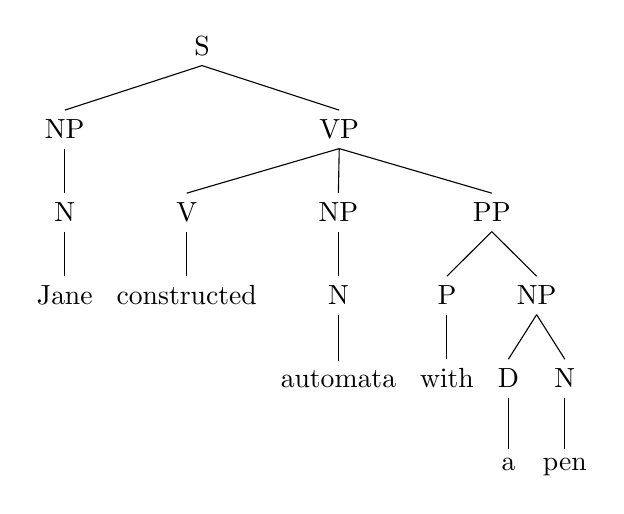
\begin{tikzpicture}[scale=1]
\Tree [.S [.NP [.N Jane ] ] [.VP [.V constructed ] [.NP [.N automata ] ] [.PP [.P with ] [.NP [.D a ] [.N pen ] ] ] ] ]
\end{tikzpicture}
\end{tcolorbox}

\paragraph{b)} my book in the man built a Jane by a pen \hfill \small{(4/20 pts)} \\

\begin{tcolorbox}
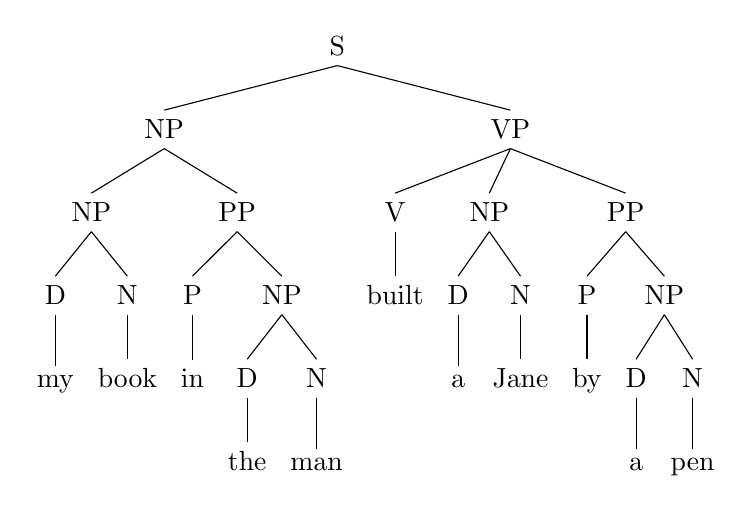
\begin{tikzpicture}[scale=1]
\Tree [.S [.NP [.NP [.D my ] [.N book ] ] [.PP [.P in ] [.NP [.D the ] [.N man ] ] ] ] [.VP [.V built ] [.NP [.D a ] [.N Jane ] ] [.PP [.P by ] [.NP [.D a ] [.N pen ] ] ] ] ]
\end{tikzpicture}
\end{tcolorbox}

\newpage

Given the CFG below, answer \textbf{c}, \textbf{d} and \textbf{e} \\

\begin{lstlisting}[style=output,mathescape=true]
S  $\to$ E
E  $\to$ E + T | E - T | T
T  $\to$ T * I | T / I | I
I  $\to$ 0 | 1 | 2 | 3 | 4 | 6 | 7 | 8 | 9
\end{lstlisting}

\paragraph{c)} Provide the left-most derivation of 7 - 4 * 3 step-by-step and plot the final parse \hfill \small{(4/20 pts)} \\
tree matching that derivation \\

\begin{tcolorbox}
$S\Rightarrow E\Rightarrow E-T\Rightarrow T-T\Rightarrow I-T\Rightarrow 7-T\Rightarrow 7-T*I\Rightarrow 7-I*I\Rightarrow 7-4*I\Rightarrow 7-4*3$ \\
! The parse tree is identical to the parse tree in part d. (I was not able to paste it here as well due to some tcolorbox error I couldn't solve)
\end{tcolorbox}



\paragraph{d)} Provide the right-most derivation of 7 - 4 * 3 step-by-step and plot the final parse \hfill \small{(4/20 pts)} \\
 tree matching that derivation \\
 
\begin{tcolorbox}
$S\Rightarrow E\Rightarrow E-T\Rightarrow E-T*I\Rightarrow E-T*3\Rightarrow E-I*3\Rightarrow E-4*3\Rightarrow T-4*3\Rightarrow I-4*3\Rightarrow 7-4*3$ \\
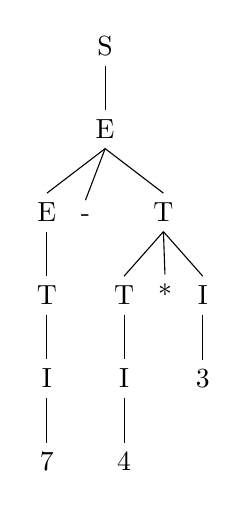
\begin{tikzpicture}[scale=1]
\Tree [.S  [.E [.E [.T [.I 7 ] ] ] [.- ] [.T [.T [.I 4 ] ] [.* ] [.I 3 ] ] ] ] 
\end{tikzpicture}
\end{tcolorbox}


\paragraph{e)} Are the derivations in \textbf{c} and \textbf{d} in the same similarity class?  \hfill \small{(4/20 pts)} \\

\begin{tcolorbox}
Yes. If we have to elaborate, we can go from c to d or from d to c by repeatedly following either a $\prec$, or an inverted $\prec$. \\
Also, we can say that if two derivations have the same parse tree then they are in the same similarity class. In this case both c and d have the same parse tree.
\end{tcolorbox}


\newpage
\section{Pushdown Automata \hfill \normalfont{(30 pts)}}

\paragraph{a)} 
Find the language recognized by the PDA given below \hfill \small{(5/30 pts)} \\

\begin{tikzpicture}[shorten >=1pt,node distance=3cm,on grid,auto]
\node[state,initial,initial text=] (q_0) {$q_0$};
\node[state] (q_1) [right=of q_0] {$q_1$};
\node[state] (q_2) [above right=of q_1] {$q_2$};
\node[state] (q_3) [below right=of q_1] {$q_3$};
\node[state,accepting](q_4) [right=of q_2] {$q_4$};
\node[state](q_5) [right=of q_3] {$q_5$};
\node[state,accepting](q_6) [right=of q_5] {$q_6$};
\path[->]

(q_0) edge node {$\varepsilon,\varepsilon \to \#$} (q_1)
(q_1) edge [loop below] node {$x,\varepsilon \to x$} (q_1)

%%
(q_1) edge node {$\varepsilon,\varepsilon \to \varepsilon$} (q_2)
(q_2) edge [loop above] node {$y,x \to \varepsilon$} (q_2)

(q_2) edge node {$\varepsilon,\# \to \varepsilon$} (q_4)
(q_4) edge [loop above] node {$z,\varepsilon \to \varepsilon$} (q_4)

%%%

(q_1) edge node {$\varepsilon,\varepsilon \to \varepsilon$} (q_3)
(q_3) edge [loop below] node {$y,\varepsilon \to \varepsilon$} (q_3)

(q_3) edge node {$\varepsilon,\varepsilon \to \varepsilon$} (q_5)
(q_5) edge [loop below] node {$z,x \to \varepsilon$} (q_5)

(q_5) edge node {$\varepsilon,\# \to \varepsilon$} (q_6)
;
\end{tikzpicture} \\

\begin{minipage}{0.60\textwidth}
where the transition $((q_i,\alpha,\beta),(q_j,\gamma)) $ is represented as: 
\end{minipage}
\begin{minipage}{0.30\textwidth}
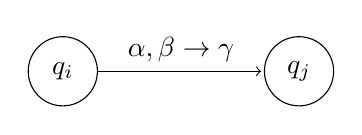
\begin{tikzpicture}[shorten >=1pt,node distance=3cm,on grid,auto]
\node[state] (q_i) {$q_i$};
\node[state] (q_j) [right=of q_i] {$q_j$};
\path[->]
(q_i) edge node {$\alpha,\beta \to \gamma$} (q_j);
\end{tikzpicture} \\
\end{minipage}


\begin{tcolorbox}
$ L=\{ x^ny^nz^m\ |\ n, m\geq 0;\ n,m\in \mathbb{N}\} \cup \{ x^ny^mz^n\ |\ n,m \geq 0;\ n,m\in \mathbb{N} \} $
\end{tcolorbox}


\paragraph{b)} 
Design a PDA to recognize language $ L=\{x^n y^{m+n} x^m \mid \; n,m \geq 0; \; n,m \in \mathbb{N}  \} $  \hfill \small{(5/30 pts)} \\

\begin{tcolorbox}

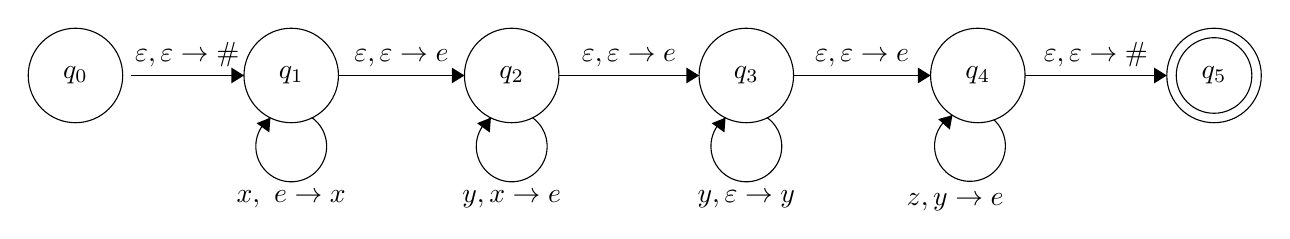
\begin{tikzpicture}[scale=0.2]
\tikzstyle{every node}+=[inner sep=0pt]
\draw [black] (3,-29) circle (3);
\draw (3,-29) node {$q_0$};
\draw [black] (16.7,-29) circle (3);
\draw (16.7,-29) node {$q_1$};
\draw [black] (30.7,-29) circle (3);
\draw (30.7,-29) node {$q_2$};
\draw [black] (45.6,-29) circle (3);
\draw (45.6,-29) node {$q_3$};
\draw [black] (60.3,-29) circle (3);
\draw (60.3,-29) node {$q_4$};
\draw [black] (75.3,-29) circle (3);
\draw (75.3,-29) node {$q_5$};
\draw [black] (75.3,-29) circle (2.4);
\draw [black] (6.5,-29) -- (13.7,-29);
\fill [black] (13.7,-29) -- (12.9,-28.5) -- (12.9,-29.5);
\draw (10.1,-28.5) node [above] {$\varepsilon,\varepsilon\rightarrow \#$};
\draw [black] (19.7,-29) -- (27.7,-29);
\fill [black] (27.7,-29) -- (26.9,-28.5) -- (26.9,-29.5);
\draw (23.7,-28.5) node [above] {$\varepsilon,\varepsilon\rightarrow e$};
\draw [black] (33.7,-29) -- (42.6,-29);
\fill [black] (42.6,-29) -- (41.8,-28.5) -- (41.8,-29.5);
\draw (38.15,-28.5) node [above] {$\varepsilon,\varepsilon\rightarrow e$};
\draw [black] (48.6,-29) -- (57.3,-29);
\fill [black] (57.3,-29) -- (56.5,-28.5) -- (56.5,-29.5);
\draw (52.95,-28.5) node [above] {$\varepsilon,\varepsilon\rightarrow e$};
\draw [black] (63.3,-29) -- (72.3,-29);
\fill [black] (72.3,-29) -- (71.5,-28.5) -- (71.5,-29.5);
\draw (67.8,-28.5) node [above] {$\varepsilon,\varepsilon\rightarrow \#$};
\draw [black] (18.023,-31.68) arc (54:-234:2.25);
\draw (16.7,-36.25) node [below] {$x,\mbox{ }e\rightarrow x$};
\fill [black] (15.38,-31.68) -- (14.5,-32.03) -- (15.31,-32.62);
\draw [black] (32.023,-31.68) arc (54:-234:2.25);
\draw (30.7,-36.25) node [below] {$y,x\rightarrow e$};
\fill [black] (29.38,-31.68) -- (28.5,-32.03) -- (29.31,-32.62);
\draw [black] (46.923,-31.68) arc (54:-234:2.25);
\draw (45.6,-36.25) node [below] {$y,\varepsilon\rightarrow y$};
\fill [black] (44.28,-31.68) -- (43.4,-32.03) -- (44.21,-32.62);
\draw [black] (61.317,-31.81) arc (47.63229:-240.36771:2.25);
\draw (58.86,-36.47) node [below] {$z,y\rightarrow e$};
\fill [black] (58.69,-31.52) -- (57.78,-31.77) -- (58.52,-32.44);
\end{tikzpicture}

\end{tcolorbox}

\newpage

\paragraph{c)} 
Design a PDA to recognize language $ L=\{x^n y^m \mid \; n < m \leq 2n; \; n,m \in \mathbb{N^+} \} $  \hfill \small{(10/30 pts)} \\
Do not use multi-symbol push/pop operations in your transitions. \\
Simulate the PDA on strings \textit{xxy} (with only one rejecting derivation) and \textit{xxyyyy} (accepting derivation) with transition tables. \\


\begin{tcolorbox}
$M=(K,\Sigma,\Gamma,\Delta,q_0,\{q_6\})$ where $K=\{q_0,q_1,q_2,q_3,q_4,q_5,q_6\}$ and $\Sigma=\{a,b\}$ \\
\begin{equation}
\begin{split}
\Delta = \{ & ((q_0,\varepsilon,\varepsilon),(q_1,\#)),\ \ (1) \\
		& ((q_1,x,\varepsilon),(q_2,x)),\ \ (2) \\
		& ((q_2,\varepsilon,\varepsilon),(q_1,x)),\ \ (3) \\
		& ((q_1,y,x),(q_3,x)),\ \ (4) \\
		& ((q_3,y,x),(q_4,\varepsilon)),\ \ (5) \\
		& ((q_4,\varepsilon,x),(q_3,\varepsilon)),\ \ (6) \\
		& ((q_3,y,x),(q_5,\varepsilon)),\ \ (7) \\
		& ((q_5,y,x),(q_3,\varepsilon)),\ \ (8) \\
		& ((q_3,\varepsilon,\#),(q_6,\varepsilon)) \} \ \ (9)
\end{split}
\end{equation}
\begin{center}
\begin{tikzpicture}[scale=0.2]
\tikzstyle{every node}+=[inner sep=0pt]
\draw [black] (3.1,-28.3) circle (3);
\draw (3.1,-28.3) node {$q_0$};
\draw [black] (23,-28.3) circle (3);
\draw (23,-28.3) node {$q_1$};
\draw [black] (23,-46.7) circle (3);
\draw (23,-46.7) node {$q_2$};
\draw [black] (55.7,-28.3) circle (3);
\draw (55.7,-28.3) node {$q_3$};
\draw [black] (55.7,-52.5) circle (3);
\draw (55.7,-52.5) node {$q_4$};
\draw [black] (55.7,-11.1) circle (3);
\draw (55.7,-11.1) node {$q_5$};
\draw [black] (75.5,-28.3) circle (3);
\draw (75.5,-28.3) node {$q_6$};
\draw [black] (75.5,-28.3) circle (2.4);
\draw [black] (6.1,-28.3) -- (20,-28.3);
\fill [black] (20,-28.3) -- (19.2,-27.8) -- (19.2,-28.8);
\draw (13.05,-27.8) node [above] {$(1)\mbox{ }\varepsilon\mbox{ }\rightarrow\mbox{ }\#$};
\draw [black] (22.178,-43.816) arc (-167.12426:-192.87574:28.345);
\fill [black] (22.18,-43.82) -- (22.49,-42.92) -- (21.51,-43.15);
\draw (20.97,-37.5) node [left] {$(2)\mbox{ }x,\mbox{ }\varepsilon\mbox{ }\rightarrow\mbox{ }x$};
\draw [black] (23.822,-31.184) arc (12.87574:-12.87574:28.345);
\fill [black] (23.82,-31.18) -- (23.51,-32.08) -- (24.49,-31.85);
\draw (25.03,-37.5) node [right] {$(3)\mbox{ }\varepsilon,\mbox{ }\varepsilon\mbox{ }\rightarrow\mbox{ }x$};
\draw [black] (26,-28.3) -- (52.7,-28.3);
\fill [black] (52.7,-28.3) -- (51.9,-27.8) -- (51.9,-28.8);
\draw (39.35,-27.8) node [above] {$(4)\mbox{ }y, \mbox{ }x\mbox{ }\rightarrow\mbox{ }x$};
\draw [black] (56.554,-13.974) arc (13.13183:-13.13183:25.203);
\fill [black] (56.55,-13.97) -- (56.25,-14.87) -- (57.22,-14.64);
\draw (57.71,-19.7) node [right] {$(7)\mbox{ }y,\mbox{ }x\mbox{ }\rightarrow\mbox{ }\varepsilon$};
\draw [black] (54.785,-25.445) arc (-165.88662:-194.11338:23.56);
\fill [black] (54.79,-25.44) -- (55.08,-24.55) -- (54.11,-24.79);
\draw (53.57,-19.7) node [left] {$(8)\mbox{ }y,\mbox{ }x\mbox{ }\rightarrow\mbox{ }\varepsilon$};
\draw [black] (56.362,-31.226) arc (10.96292:-10.96292:48.242);
\fill [black] (56.36,-31.23) -- (56.02,-32.11) -- (57,-31.92);
\draw (57.74,-40.4) node [right] {$(6)\mbox{ }\varepsilon,\mbox{ }x\mbox{ }\rightarrow\mbox{ }\varepsilon$};
\draw [black] (54.893,-49.611) arc (-166.56194:-193.43806:39.637);
\fill [black] (54.89,-49.61) -- (55.19,-48.72) -- (54.22,-48.95);
\draw (53.31,-40.4) node [left] {$(5)\mbox{ }y,\mbox{ }x\mbox{ }\rightarrow\mbox{ }\varepsilon$};
\draw [black] (58.7,-28.3) -- (72.5,-28.3);
\fill [black] (72.5,-28.3) -- (71.7,-27.8) -- (71.7,-28.8);
\draw (65.6,-27.8) node [above] {$(9)\mbox{ }\varepsilon,\mbox{ }\#\mbox{ }\rightarrow\mbox{ }\varepsilon$};
\end{tikzpicture}
\vspace{4cm}
\end{center}
\begin{table}[H]
\begin{tabular}{cccc}
{\ul \textbf{State}} & {\ul \textbf{Unread Input}} & {\ul \textbf{Stack}} & {\ul \textbf{Transition}} \\
$q_0$ & xxy & e & - \\
$q_1$ & xxy & \# & 1 \\
$q_2$ & xy & x\# & 2 \\
$q_1$ & xy & xx\# & 3 \\
$q_2$ & y & xxx\# & 2 \\
$q_1$ & y & xxxx\# & 3 \\
$q_3$ & e & xxxx\# & 4 
\end{tabular}
\end{table}
Input xxy is not accepted.
\begin{table}[H]
\begin{tabular}{cccc}
{\ul \textbf{State}} & {\ul \textbf{Unread Input}} & {\ul \textbf{Stack}} & {\ul \textbf{Transition}} \\
$q_0$ & xxyyyy & e & - \\
$q_1$ & xxyyyy & \# & 1 \\
$q_2$ & xyyyy & x\# & 2 \\
$q_1$ & xyyyy & xx\# & 3 \\
$q_2$ & yyyy & xxx\# & 2 \\
$q_1$ & yyyy & xxxx\# & 3 \\
$q_3$ & yyy & xxxx\# & 4 \\
$q_4$ & yy & xxx\# & 5 \\
$q_3$ & yy & xx\# & 6 \\
$q_5$ & y & x\# & 7 \\
$q_3$ & e & \# & 8 \\
$q_6$ & e & e & 9 
\end{tabular}
\end{table}
Input xxyyyy is accecpted.
\end{tcolorbox}
\vspace{11cm}

\paragraph{d)} Given two languages $L'$ and $L$ as $L'=\{w \mid \; w\in L; \; |w|=4n+2 \; for\; n\in \mathbb{N} \}$
\hfill \small{(10/30 pts)} \\
If $L$ is a CFL, show that $L'$ is also a CFL by constructing an automaton for $L'$ in terms of another automaton that recognizes $L$. \\


\begin{tcolorbox}
The given language $L'=L \cap L''$ where $L''=\{w\ |\ |w|=4n+2\ for\ n\in \mathbb{N} \}$. \\
Lets say that $L=L(M_1)$ for some pushdown automaton $M_1=(K_1,\Sigma,\Gamma_1,\Delta_1,s_1,F_1)$. \\
Furthermore, we can easily show that $L''$ is a regular language by constructing a deterministic finite automaton as follows: \\
Let $M_2=(K_2,\Sigma,\delta,s_2,F_2)$ where 
$K_2=\{q_0,q_1,q_2,q_3\},\ \Sigma=\{ \sigma_1,\ ...,\ \sigma_n \},\ s_2=q_0,\ F_2=\{q_2\}$
\begin{equation}
\begin{split}
\delta(q_0,\sigma_i)&=q_1\\
\delta(q_1,\sigma_i)&=q_2 \\
\delta(q_2,\sigma_i)&=q_3 \\
\delta(q_3,\sigma_i)&=q_0\ \text{ for any $\sigma_i \in \Sigma$}
\end{split}
\end{equation}
and we say that $L''=L(M_2)$. To illustrate, 
\begin{center}
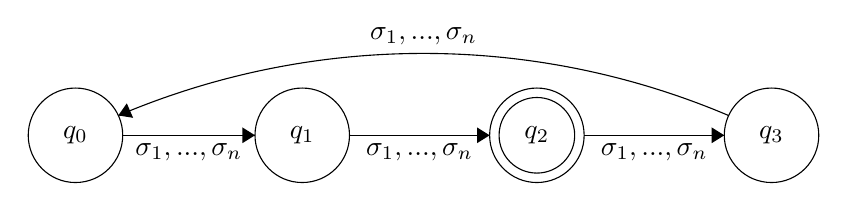
\begin{tikzpicture}[scale=0.2]
\tikzstyle{every node}+=[inner sep=0pt]
\draw [black] (11.6,-24.5) circle (3);
\draw (11.6,-24.5) node {$q_0$};
\draw [black] (26,-24.5) circle (3);
\draw (26,-24.5) node {$q_1$};
\draw [black] (40.9,-24.5) circle (3);
\draw (40.9,-24.5) node {$q_2$};
\draw [black] (40.9,-24.5) circle (2.4);
\draw [black] (55.8,-24.5) circle (3);
\draw (55.8,-24.5) node {$q_3$};
\draw [black] (14.6,-24.5) -- (23,-24.5);
\fill [black] (23,-24.5) -- (22.2,-24) -- (22.2,-25);
\draw (18.8,-25) node [below] {$\sigma_1,...,\sigma_n$};
\draw [black] (29,-24.5) -- (37.9,-24.5);
\fill [black] (37.9,-24.5) -- (37.1,-24) -- (37.1,-25);
\draw (33.45,-25) node [below] {$\sigma_1,...,\sigma_n$};
\draw [black] (43.9,-24.5) -- (52.8,-24.5);
\fill [black] (52.8,-24.5) -- (52,-24) -- (52,-25);
\draw (48.35,-25) node [below] {$\sigma_1,...,\sigma_n$};
\draw [black] (14.324,-23.244) arc (113.01305:66.98695:49.562);
\fill [black] (14.32,-23.24) -- (15.26,-23.39) -- (14.86,-22.47);
\draw (33.7,-18.8) node [above] {$\sigma_1,...,\sigma_n$};
\end{tikzpicture}
\end{center}

We need to construct a pushdown automaton by combining these two automata ($M_1,M_2$) into a single pushdown automaton so that we can show $L'$ is a context free language. Let this automaton be $M=(K,\Sigma,\Gamma,\Delta,s,F)$, \\
\begin{equation}
\begin{split}
K & = K_1 \text{x} K_2 \\
\Gamma & = \Gamma_1 \\
s & = (s_1,s_2) \\
F & = F_1 \text{x} F_2 
\end{split}
\end{equation} 
For each transition of form $((q_x,\sigma,\beta),(p_x,\gamma))\in \Delta_1$, and for each state $q_0,q_1,q_2,q_3 \in K_2$ we add the following transition to $\Delta$: 
$$(((q_x,q_i), \sigma,\beta),((p_x,\delta(q_i,\sigma))),\gamma)\ \ \text{ for any $\sigma \in \Sigma$ and \underline{for each} $q_i \in K_2=\{q_0,q_1,q_2,q_3\}$}$$
For each transition of form $((q_x,e,\beta),(p_x,\gamma))\in \Delta_1$, and for each  state $q_0,q_1,q_2,q_3 \in K_2$ we add the following transition to $\Delta$: 
$$(((q_x,q_i), e,\beta),((p_x,q_i),\gamma)\ \ \text{ for any $\sigma \in \Sigma$ and \underline{for each} $q_i \in K_2=\{q_0,q_1,q_2,q_3\}$}$$ 
\begin{equation}
\begin{split}
\Delta = \text{\{} &((q_x,q_0), \sigma,\beta),((p_x,q_1)),\gamma) \\
	        &((q_x,q_1), \sigma,\beta),((p_x,q_2)),\gamma) \\
	        &((q_x,q_2), \sigma,\beta),((p_x,q_3)),\gamma) \\
	        &((q_x,q_3), \sigma,\beta),((p_x,q_0)),\gamma) \text{\} } \text{ for every $\beta,\gamma \in \Gamma_1$ } \\
	        &\text{ and so on... (there may need to be additions to them depending on $M_1$)} 
\end{split}
\end{equation} 

We now can easily see that $w\in L(M)$ if and only if $w\in L(M_1)\cap L(M_2)$. \\
Meaning, $L(M)=L\cap L''$ and $L'=L(M)$.
\end{tcolorbox}







\newpage
\section{Closure Properties \hfill \normalfont{(20 pts)}}

Let $L_1$ and $L_2$ be context-free languages which are not regular, and let $L_3$ be a regular language. Determine whether the following languages are necessarily CFLs or not. If they need to be context-free, explain your reasoning. If not, give one example where the language is a CFL and a counter example where the language is not a CFL. \\

\paragraph{a)} $L_4 = L_1 \cap (L_2 \setminus L_3)$ \hfill \small{(10/20 pts)} \\

\begin{tcolorbox}
$L_4$ is not necessarily context-free. \\
$(L_2 \setminus L_3)$ this part can be written as $(L_2 \cap L_3')$. Since $L_3$ is a regular language we know from the second chapter that regular languages are closed under complementation, meaning $L_3'$ is also regular. That's why $(L_2 \cap L_3')$ can be interpreted as the intersection of a context-free language and a regular language. From the textbook Theorem 3.5.2 we know that intersection of a context-free language and a regular language is context-free language. 
\begin{equation}
\begin{split}
L_4 &  = \ L_1 \cap (L_2 \cap L_3') \\
       &  = \text{ Context-free $\cap$ (Context-free $\cap$ Regular)} \\
       &  = \text{ Context-free $\cap$ Context-free}\ \neq \text{ Context-free\ \ (not necessarily)} \\
\end{split}
\end{equation}
Not necessarily context-free because the class of context-free languages is not closed under intersection. \\
\textbf{CFL example : } \\
$L_1=a^*b^*$ is both regular and context-free because the class of regular languages is the proper subset of the class of context-free langauges. $L_2=\{a^nb^n\ |\ n\geq 0,\ n\in \mathbb{N}  \}$. $L_1\cap L_2=\{a^nb^n\ |\ n\geq 0,\ n\in \mathbb{N}  \}$ which is a context-free language. \\
\textbf{Counter example : } \\
$L_1=\{a^mb^nc^n\ |\ n,m\geq 0;\ n,m\in \mathbb{N} \}$ and $L_2=\{a^nb^nc^m\ |\ n,m\geq 0;\ n,m\in \mathbb{N} \}$. $L_1\cap L_2=\{a^nb^nc^n\ |\ n\geq 0,\ n\in \mathbb{N} \}$ which is not a context free language. \\ \\
Therefore $L_4$ is not necessarily context-free.
\end{tcolorbox}

\paragraph{b)} $L_5 = (L_1 \cap L_3)\text{*}$ \hfill \small{(10/20 pts)} \\

\begin{tcolorbox}
$L_5$ is context-free. \\
From the textbook Theorem 3.5.2 we know that intersection of a context-free language and a regular language is context-free language.\\
In this question we see that $L_1\cap L_3$ is context-free since $L_1$ is context-free and $L_3$ is regular. Context free languages are closed under Kleene star operation. Meaning, 
\begin{equation}
\begin{split}
L_5 &  = \ (L_1 \cap L_3)^* \\
       &  = \text{ (Context-free)$^*$} \\
       &  = \text{ Context-free } \\
\end{split}
\end{equation}
Therefore $L_5$ is indeed a context-free language.
\end{tcolorbox}





\newpage
\section{Pumping Theorem \hfill \normalfont{(20 pts)}}

\paragraph{a)} Show that $L=\{a^n m^n t^i \mid \; n\leq i \leq 2n\}$ is not a Context Free Language \hfill \small{(10/20 pts)} \\
using Pumping Theorem for CFLs. \\

\begin{tcolorbox}
Assume that language $L$ is a context-free language then the pumping theorem would apply. \\
Given pumping constant $K\geq1$,
$$w=a^Km^{K}t^K\in L,\quad |w|=3K>K$$
Then by the pumping theorem w can be written as follows,
$$w=uvxyz \text{ such that } vy\neq e,\ w'=|vxy|\leq K$$
Now we have two general cases, \\
\textbf{\underline{$w'$ contains only 1 symbol}} \\
$w'=a^j$ \\
$w'=m^j$ \\
$w'=t^j$ 
where $1\leq j\leq K$ \\
\textbf{\underline{$w'$ contains 2 symbols}} \\
$w'=a^jm^l$ \\
$w'=m^jt^l$ where $1\leq j+l \leq K$ \\
\textbf{\underline{$w'$ cannot contain $at$ or $amt$ because $|w'|\leq K$}} \\ 
By the pumping theorem we can say that $uv^nxy^nz\in L$ must be true for all $n\geq 0$, \\
\textbf{\underline{Case 1 :}} \\
$w'=a^j$ where $1\leq j\leq K$. Take n=0, 
$$uxz=a^{K'}m^{K}t^{K}   \text{, where }  K'<K \text{ therefore } uxz\notin L$$
$w'=m^j$ where $1\leq j\leq K$. Take n=0, 
$$uxz=a^{K}m^{K'}t^{K}  \text{, where } K'<K \text{ therefore } uxz\notin L$$
$w'=t^j$ where $1\leq j\leq K$. Take n=0, 
$$uxz=a^{K}m^{K}t^{K'}  \text{, where } K'<K \text{ therefore } uxz\notin L$$
\textbf{\underline{Case 2 :}} \\
$w'=a^jm^l$ where $1\leq j+l\leq K$. Take n=0, 
$$uxz=a^{K'}m^{K''}t^{K}  \text{, where } K'<K \text{ and } K''<K \text{ therefore } uxz\notin L$$
$w'=m^jt^l$ where $1\leq j+l\leq K$. Take n=0, 
$$uxz=a^{K}m^{K'}t^{K''} \text{, where } K'<K \text{ and } K''<K \text{ therefore } uxz\notin L$$ \\
There exists a contradiction with the assumption we made. \\
Therefore, L is not context-free.
\end{tcolorbox}


\paragraph{b)} Show that $L=\{a^n b^{2n} a^n \mid \; n \in \mathbb{N+} \}$ is not a Context Free Language \hfill \small{(10/20 pts)} \\
using Pumping Theorem for CFLs. \\

\begin{tcolorbox}
Assume that language $L$ is a context-free language then the pumping theorem would apply. \\
Given pumping constant $K\geq1$,
$$w=a^Kb^{2K}a^K\in L,\quad |w|=4K>K$$
Then by the pumping theorem w can be written as follows,
$$w=uvxyz \text{ such that } vy\neq e,\ w'=|vxy|\leq K$$
Now we have two general cases, \\
\textbf{\underline{$w'$ contains only 1 symbol}} \\
$w'=a^j$ \\
$w'=b^j$ where $1\leq j\leq K$ \\
\textbf{\underline{$w'$ contains 2 symbols}} \\
$w'=a^jb^l$ \\
$w'=b^ja^l$ where $1\leq j+l \leq K$ \\
\textbf{\underline{w' cannot contain $aa$ or $aba$ because $|w'|\leq K$}} \\ 
By the pumping theorem we can say that $uv^nxy^nz\in L$ must be true for all $n\geq 0$, \\
\textbf{\underline{Case 1 :}} \\
$w'=a^j$ where $1\leq j\leq K$. Take n=0, 
$$uxz=a^{K'}b^{2K}a^K \text{ or } uxz=a^{K}b^{2K}a^{K'} \text{, for both of the cases } K'<K \text{ therefore } uxz\notin L$$
$w'=b^j$ where $1\leq j\leq K$. Take n=0, 
$$uxz=a^{K}b^{T}a^K  \text{, where } T<2K \text{ therefore } uxz\notin L$$
\textbf{\underline{Case 2 :}} \\
$w'=a^jb^l$ where $1\leq j+l\leq K$. Take n=0, 
$$uxz=a^{K'}b^{T}a^K \text{, where } K'<K \text{ and } T<2K \text{ therefore } uxz\notin L$$
$w'=b^ja^l$ where $1\leq j+l\leq K$. Take n=0, 
$$uxz=a^{K}b^{T}a^{K'}\text{, where } K'<K \text{ and } T<2K \text{ therefore } uxz\notin L$$\\
There exists a contradiction with the assumption we made. \\
Therefore, L is not context-free.
\end{tcolorbox}

\end{document}

​
